\section{LIYANA MAJDAH RAHMA 1174039}
\subsection{Teori}
\subsubsection{Soal No. 1}
\hfill \break
Apa itu fungsi library matplotlib?

\hfill \break
Matplotlib merupakan salah satu library Python 2D yang dapat menghasilkan plot dengan kualitas yang tinggi dalam berbagai format dan dapat digunakan di berbagai platform. Matplotlib berfungsi sebagai pembuat grafik di berbagai platform, seperti Python dan Jupyter. Grafik yang dibuat menggunakan Matplotlib bisa dibuat dalam berbagai bentuk, seperti grafik garis, batang, lingkaran, histogram, dan sebagainya.

\subsubsection{Soal No. 2}
\hfill \break
Jelaskan langkah-langkah membuat sumbu X dan Y di matplotlib!

\begin{enumerate}
	\item Pertama import library Matplotlib.	
	\lstinputlisting[firstline=2, lastline=2]{src/6/Teori/1174039/1174039.py}
	
	\item Buat variabel x yang menampung list untuk sumbu x dan variabel y yang menampung list untuk sumbu y.	
	\lstinputlisting[firstline=4, lastline=5]{src/6/Teori/1174039/1174039.py}
	
	\item Panggil fungsi plot dan isi parameter pertama dengan variabel x dan parameter kedua dengan variabel y.
	\lstinputlisting[firstline=7, lastline=7]{src/6/Teori/1174039/1174039.py}	

	\item Lalu panggil plot tadi dengan memanggil fungsi show.
	\lstinputlisting[firstline=9, lastline=9]{src/6/Teori/1174039/1174039.py}
	
\end{enumerate}
\hfill \break
\textbf{Kode Program}

\lstinputlisting[caption = Kode program membuat diagram menggunakan Matplotlib., firstline=2, lastline=9]{src/6/Teori/1174039/1174039.py}

\hfill \break
\textbf{Hasil Compile}

\begin{figure}[H]
	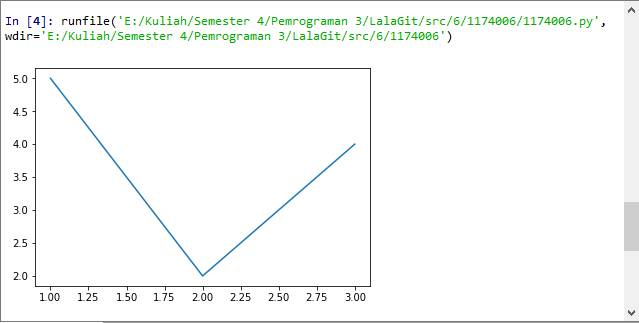
\includegraphics[width=12cm]{figures/6/Teori/1174039/2.png}
	\centering
	\caption{Hasil compile membuat diagram menggunakan Matplotlib.}
\end{figure}
 
\subsubsection{Soal No. 3}
\hfill \break
Jelaskan bagaimana perbedaan fungsi dan cara pakai untuk berbagai jenis(bar, histogram ,scatter ,line, dll) jenis plot di matplotlib!

\begin{enumerate}
	\item \textbf{Bar Graph}
	
	Perbedaan bar graph dengan jenis plot yang lain adalah bar graph menggunakan bar atau batang-batang untuk membandingkan data di antara berbagai kategori.
	
	\textbf{Kode Program}
	
	\lstinputlisting[caption = Kode program membuat bar graph menggunakan Matplotlib., firstline=2, lastline=9]{src/6/Teori/1174039/1174039.py}
	
	\textbf{Hasil Compile}
	
	\begin{figure}[H]
		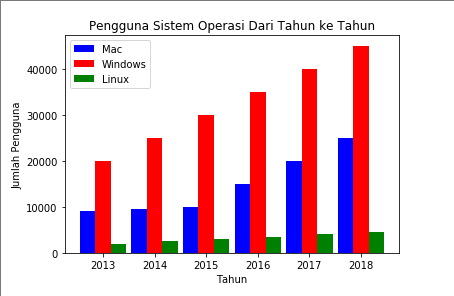
\includegraphics[width=12cm]{figures/6/Teori/1174039/bar.png}
		\centering
		\caption{Hasil compile membuat bar graph menggunakan Matplotlib.}
	\end{figure}
	
	\item \textbf{Histogram}
	
	Perbedaan histogram dengan jenis plot yang lain adalah histogram akan membuat plot dimana plot yang dimunculkan merupakan gabungan dari beberapa data yang telah dikelompokkan.
	
	\textbf{Kode Program}
	
	\lstinputlisting[caption = Kode program membuat histogram menggunakan Matplotlib., firstline=29, lastline=36]{src/6/Teori/1174039/1174039.py}
	
	\textbf{Hasil Compile}
	
	\begin{figure}[H]
		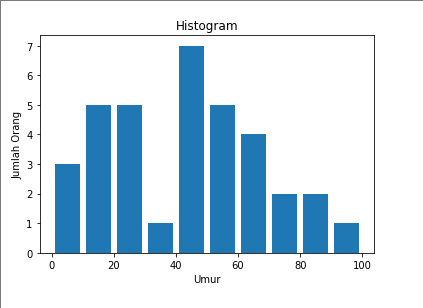
\includegraphics[width=12cm]{figures/6/Teori/1174039/histogram.png}
		\centering
		\caption{Hasil compile membuat histogram menggunakan Matplotlib.}
	\end{figure}
	
	\item \textbf{Scatter Plot}
	
	Perbedaan scatter plot dengan jenis plot lain adalah scatter plot menampilkan data sebagai kumpulan titik, masing-masing memiliki nilai satu variabel yang menentukan posisi pada sumbu horizontal dan nilai variabel lain menentukan posisi pada sumbu vertikal.
	
	\textbf{Kode Program}
	
	\lstinputlisting[caption = Kode program membuat scatter plot menggunakan Matplotlib., firstline=40, lastline=53]{src/6/Teori/1174039/1174039.py}
	
	\textbf{Hasil Compile}
	
	\begin{figure}[H]
		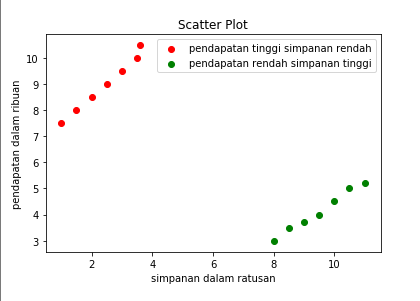
\includegraphics[width=12cm]{figures/6/Teori/1174039/scatter.png}
		\centering
		\caption{Hasil compile membuat scatter plot menggunakan Matplotlib.}
	\end{figure}
	
	\item \textbf{Area Plot}
	
	Perbedaan area plot dengan jenis plot lain adalah area plot digunakan untuk melacak perubahan dari waktu ke waktu untuk dua atau lebih kelompok terkait yang membentuk satu kategori secara keseluruhan.
	
	\textbf{Kode Program}
	
	\lstinputlisting[caption = Kode program membuat diagram menggunakan Matplotlib., firstline=57, lastline=76]{src/6/Teori/1174039/1174039.py}
	
	\textbf{Hasil Compile}
	
	\begin{figure}[H]
		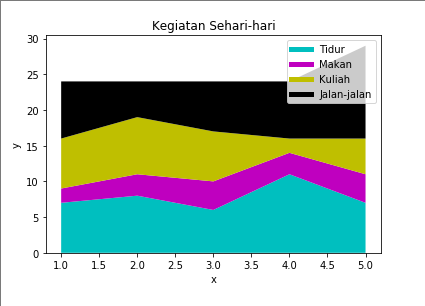
\includegraphics[width=12cm]{figures/6/Teori/1174039/area.png}
		\centering
		\caption{Hasil compile membuat diagram menggunakan Matplotlib.}
	\end{figure}
	
	\item \textbf{Pie Plot}
	
	Perbedaan pie plot dengan jenis plot lain adalah pie plot digunakan untuk menunjukkan persentase atau data proporsional di mana setiap potongan pie mewakili kategori.
	
	\textbf{Kode Program}
	
	\lstinputlisting[caption = Kode program membuat Pie Plot menggunakan Matplotlib., firstline=80, lastline=101]{src/6/Teori/1174039/1174039.py}
	
	\textbf{Hasil Compile}
	
	\begin{figure}[H]
		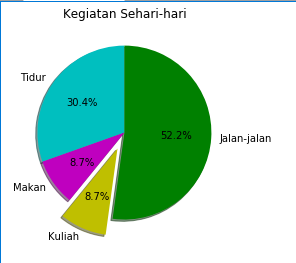
\includegraphics[width=9cm]{figures/6/Teori/1174039/pie.png}
		\centering
		\caption{Hasil compile membuat Pie Plot menggunakan Matplotlib.}
	\end{figure}
	
	\item \textbf{Line Graph}
	
	Perbedaan line graph dengan jenis plot lain adalah line graph menampilkan diagram dalam bentuk garis.
	
	\textbf{Kode Program}
	
	\lstinputlisting[caption = Kode program membuat diagram menggunakan Matplotlib., firstline=105, lastline=113]{src/6/Teori/1174039/1174039.py}
	
	\textbf{Hasil Compile}
	
	\begin{figure}[H]
		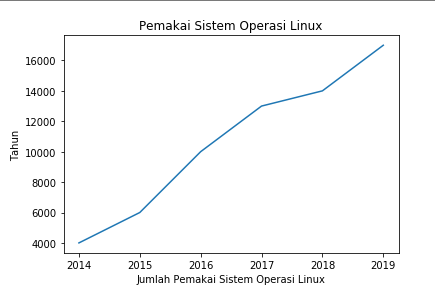
\includegraphics[width=12cm]{figures/6/Teori/1174039/line.png}
		\centering
		\caption{Hasil compile membuat diagram menggunakan Matplotlib.}
	\end{figure}
	
\end{enumerate}

\subsubsection{Soal No. 4}
\hfill \break
Jelaskan bagaimana cara menggunakan legend dan label serta kaitannya dengan fungsi tersebut!

\begin{enumerate}
	\item Untuk menggunakan legend definisikan parameter label di tiap fungsi plot. Parameter label digunakan untuk memberikan label pada line sebagai pembeda antar line.
	
	\lstinputlisting[caption = Kode program menggunakan parameter label dengan Matplotlib., firstline=123, lastline=124]{src/6/Teori/1174039/1174039.py}
	
	\item Kemudian panggil fungsi legend.
	
	\lstinputlisting[caption = Kode program memanggil fungsi legend dengan Matplotlib., firstline=128, lastline=128]{src/6/Teori/1174039/1174039.py}
\end{enumerate}

\hfill \break
\textbf{Kode Program}

\lstinputlisting[caption = Kode program membuat diagram menggunakan Matplotlib., firstline=117, lastline=130]{src/6/Teori/1174039/1174039.py}

\hfill \break
\textbf{Hasil Compile}

\begin{figure}[H]
	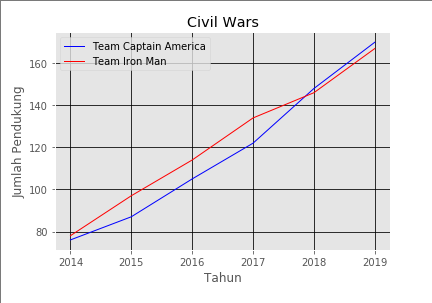
\includegraphics[width=12cm]{figures/6/Teori/1174039/4.png}
	\centering
	\caption{Hasil compile membuat diagram menggunakan Matplotlib.}
\end{figure}

\subsubsection{Soal No. 5}
\hfill \break
Jelaskan apa fungsi dari subplot di matplotlib, dan bagaimana cara kerja dari fungsi subplot, sertakan ilustrasi dan gambar sendiri dan apa parameternya jika ingin menggambar plot dengan 9 subplot di dalamnya!

\hfill \break
Fungsi subplot adalah untuk membuat beberapa plot di dalam satu gambar.
\hfill \break
Cara kerja subplot, yaitu fungsi subplot memiliki parameter pertama adalah jumlah kolom, parameter kedua adalah jumlah baris, dan parameter ketiga adalah index plot keberapanya.

\hfill \break
\textbf{Kode Program}

\lstinputlisting[caption = Kode program membuat subplot menggunakan Matplotlib., firstline=134, lastline=146]{src/6/Teori/1174039/1174039.py}

\hfill \break
\textbf{Hasil Compile}

\begin{figure}[H]
	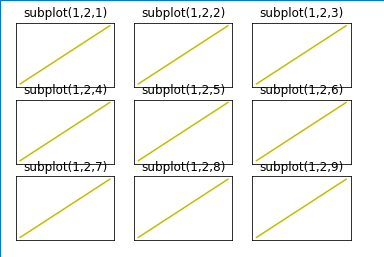
\includegraphics[width=12cm]{figures/6/Teori/1174039/subplot.png}
	\centering
	\caption{Hasil compile membuat subplot menggunakan Matplotlib.}
\end{figure}

\subsubsection{Soal No. 6}
\hfill \break
Sebutkan semua parameter color yang bisa digunakan (contoh:  m,c,r,k,...  dkk)!

\begin{itemize}
	\item 'b' (blue)
	\item 'g' (green)
	\item 'r' (red)
	\item 'c' (cyan)
	\item 'm' (magenta)
	\item 'y' (yellow)
	\item 'k' (black)
	\item 'w' (white)
\end{itemize}

\subsubsection{Soal No. 7}
\hfill \break
Jelaskan bagaimana cara kerja dari fungsi hist, sertakan ilustrasi dan gambar sendiri!

\hfill \break
Cara kerja dari fungsi hist yaitu fungsi hist akan menerima parameter yang diberikan, kemudian fungsi hist akan dieksekusi sesuai dengan parameter yang diberikan.

\hfill \break
\textbf{Kode Program}

\lstinputlisting[caption = Kode program membuat diagram menggunakan Matplotlib., firstline=150, lastline=157]{src/6/Teori/1174039/1174039.py}

\hfill \break
\textbf{Hasil Compile}

\begin{figure}[H]
	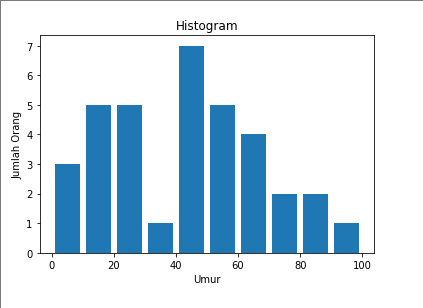
\includegraphics[width=12cm]{figures/6/Teori/1174039/histogram.png}
	\centering
	\caption{Hasil compile membuat diagram menggunakan Matplotlib.}
\end{figure}

\subsubsection{Soal No. 8}
\hfill \break
 Jelaskan lebih mendalam tentang parameter dari fungsi pie diantaranya labels, colors, startangle, shadow, explode, autopct!
 
 \begin{itemize}
 	\item labels : untuk memberikan label di tiap persentase.
 	\item colors : untuk memberikan warna di tiap persentase.
 	\item startangle : untuk memutar plot sesuai dengan derajat yang ditentukan.
 	\item shadow : untuk memberikan bayangan pada plot.
 	\item explode : untuk memisahkan antar tiap potongan pie pada plot.
 	\item autopct : untuk menentukan jumlah angka dibelakang koma.
 \end{itemize}

\subsection{Praktek}
\subsubsection{Soal No. 1}
\hfill \break
Buatlah librari fungsi (file terpisah/library dengan nama NPMbar.py) untuk plot dengan jumlah subplot adalah NPM mod 3 + 2!

\subsubsection{Soal No. 2}
\hfill \break
Buatlah librari fungsi (file terpisah/library dengan nama NPMscatter.py) untuk plot dengan jumlah subplot NPM mod 3 + 2!

\subsubsection{Soal No. 3}
\hfill \break
Buatlah librari fungsi (file terpisah/library dengan nama NPMpie.py) untuk plot dengan jumlah subplot NPM mod 3 + 2!

\subsubsection{Soal No. 4}
\hfill \break
Buatlah librari fungsi (file terpisah/library dengan nama NPMplot.py) untuk plot dengan jumlah subplot NPM mod 3 + 2


\subsection{Penanganan Error}
Tuliskan  peringatan  error  yang  didapat  dari  mengerjakan  praktek  keenam  ini, dan  jelaskan  cara  penanganan  error  tersebut. dan  Buatlah  satu  fungsi  yang menggunakan try except untuk menanggulangi error tersebut.

\section{Rangga Putra Ramdhani}
\subsection{Apa itu fungsi library matplotlib?}
Library Matplotlib berfungsi untuk membuat visualisasi yang kuat dalam menjelaskan suatu data dalam bentuk diagram dan grafik. 
Contoh grafik yang dapat digambarkan menggunakan Matplotlib adalah :
\begin{itemize}
    \item Grafik Biasa 
    \item Grafik Polar
    \item Chart
    \item Dan yang lainnya
\end{itemize}

\subsection{Jelaskan langkah-langkah membuat sumbu X dan Y di matplotlib}
Langkah langkah membuat Sumbu X dan Y adalah sebagai berikut :
\begin{itemize}
    \item Buat variabel x dan Y
    \item Masukkan nilai dari setiap variabel
    \lstinputlisting[firstline=12, lastline=13]{src/6/Teori/1174056/1174056.py}
    \item Deklarasikan nama dari sumbu x dan y 
    \lstinputlisting[firstline=16, lastline=17]{src/6/Teori/1174056/1174056.py}
\end{itemize}

Setelah dibuat, begini lah hasilnya
\begin{figure}[H]
	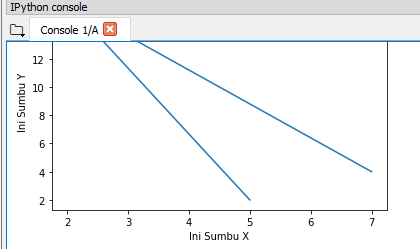
\includegraphics[width=9cm]{figures/6/Teori/1174056/1.png}
	\caption{Hasil membuat sumbu x dan y}
	\centering
\end{figure}

\subsection{Jelaskan bagaimana perbedaan fungsi dan cara pakai untuk berbagai jenis(bar,histogram,scatter,line dll) jenis plot di matplotlib}
Perbedaan fungsi dapat dilihat sebagai berikut :
\begin{itemize}
    \item Graph\linebreak
    Fungsi graph digunakan untuk membuat visualisasi berupa grafik.
    cara pakainya adalah sebagai berikut :
    \lstinputlisting[caption = fungsi untuk membuat graph., firstline=10, lastline=18]{src/6/Teori/1174056/1174056.py}
    hasilnya adalah sebagai berikut:
    \begin{figure}[H]
        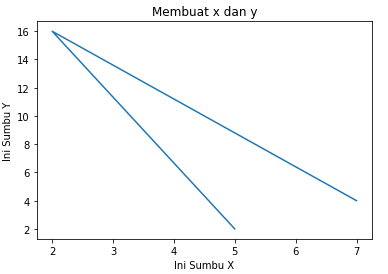
\includegraphics[width=9cm]{figures/6/Teori/1174056/3graph.png}
        \caption{Hasil graph}
        \centering
    \end{figure}

    \item Bar\linebreak 
    Fungsi Bar digunakan untuk membuat visualisasi berupa diagram batang yang berhimpit.
    Cara Pakainya adalah sebagai berikut :
    \lstinputlisting[caption = fungsi untuk membuat bar., firstline=22, lastline=32]{src/6/Teori/1174056/1174056.py}
    hasilnya adalah sebagai berikut:
    \begin{figure}[H]
        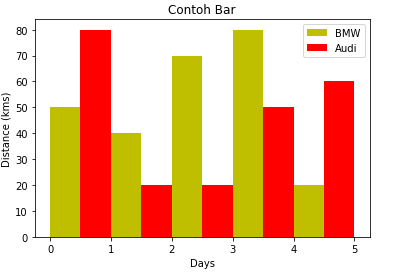
\includegraphics[width=9cm]{figures/6/Teori/1174056/3bar.png}
        \caption{Hasil bar}
        \centering
    \end{figure}

    \item Histogram\linebreak
    Fungsi Histogram digunakan untuk membuat visualisasi berupa diagram batang yang tidak berhimpit.
    Cara Pakainya adalah sebagai berikut :
    \lstinputlisting[caption = fungsi untuk membuat histogram., firstline=35, lastline=42]{src/6/Teori/1174056/1174056.py}
    hasilnya adalah sebagai berikut:
    \begin{figure}[H]
        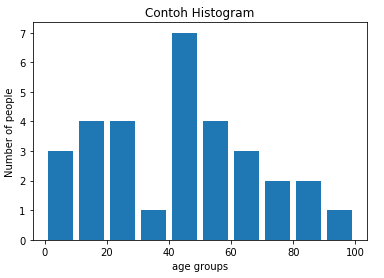
\includegraphics[width=9cm]{figures/6/Teori/1174056/3histogram.png}
        \caption{Hasil histogram}
        \centering
    \end{figure}

    \item Scatter\linebreak
    Fungsi Scatter digunakan untuk membuat visualisasi berupa titik titik.
    Cara Pakainya adalah sebagai berikut :
    \lstinputlisting[caption = fungsi untuk membuat scatter., firstline=45, lastline=58]{src/6/Teori/1174056/1174056.py}
    hasilnya adalah sebagai berikut:
    \begin{figure}[H]
        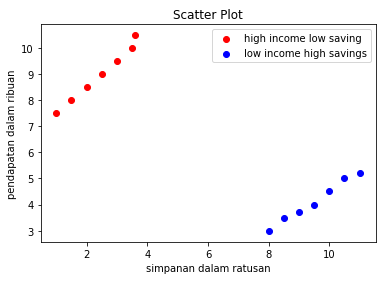
\includegraphics[width=9cm]{figures/6/Teori/1174056/3scatter.png}
        \caption{Hasil scatter}
        \centering
    \end{figure}

    \item Area plot\linebreak
    Fungsi Area plot digunakan untuk membuat visualisasi berupa area.
    Cara Pakainya adalah sebagai berikut :
    \lstinputlisting[caption = fungsi untuk membuat area plot., firstline=61, lastline=80]{src/6/Teori/1174056/1174056.py}
    hasilnya adalah sebagai berikut:
    \begin{figure}[H]
        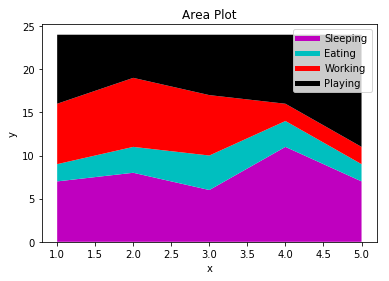
\includegraphics[width=9cm]{figures/6/Teori/1174056/3areaplot.png}
        \caption{Hasil area plot}
        \centering
    \end{figure}

    \item Pie\linebreak
    Fungsi Pie digunakan untuk membuat visualisasi berupa diagram lingkaran.
    Cara Pakainya adalah sebagai berikut :
    \lstinputlisting[caption = fungsi untuk membuat pie., firstline=83, lastline=104]{src/6/Teori/1174056/1174056.py}
    hasilnya adalah sebagai berikut:
    \begin{figure}[H]
        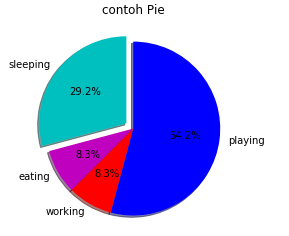
\includegraphics[width=9cm]{figures/6/Teori/1174056/3pie.png}
        \caption{Hasil pie}
        \centering
    \end{figure}
    
\end{itemize}

\subsection{Jelaskan bagaimana cara menggunakan legend dan label serta kaitannya dengan fungsi tersebut}
Fungsi legend digunakan untuk menjelaskan makna dari objek berupa titik atau garis di dalam diagram.
cara menggunakan legend adalah 
\lstinputlisting[caption = fungsi untuk membuat legend., firstline=24, lastline=28]{src/6/Teori/1174056/1174056.py}
contoh legend :
\begin{figure}[H]
    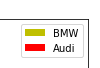
\includegraphics[width=9cm]{figures/6/Teori/1174056/4legend.png}
    \caption{contoh legend}
    \centering
\end{figure}

\subsection{Jelaskan apa fungsi dari subplot di matplotlib, dan bagaimana cara kerja dari fungsi subplot, sertakan ilustrasi dan gambar sendiri dan apa parameternya jika ingin menggambar plot dengan 9 subplot di dalamnya}
Subplot berfungsi untuk menggabungkan beberapa plot kedalam satu figure
cara kerjanya adalah sebagai berikut
\lstinputlisting[caption = cara kerja subplot., firstline=108, lastline=134]{src/6/Teori/1174056/1174056.py}
Parameter yang digunakan ketika ingin membuat 9 subplot terdiri dari (331) sampai (339). karena posisi subplot dilihat dengan melihat tinggi,lebar,urutan
hasil dari subplot adalah
\begin{figure}[H]
    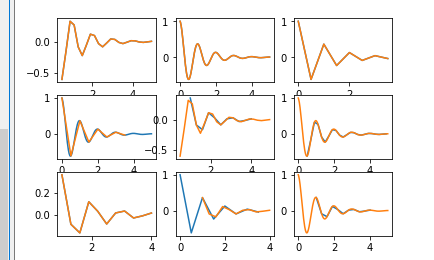
\includegraphics[width=9cm]{figures/6/Teori/1174056/5subplot.png}
    \caption{hasil subplot}
    \centering
\end{figure}

\subsection{Sebutkan semua parameter color yang bisa digunakan}
Parameter color yang bisa digunakan antara lain RGB dan CMYK
\begin{itemize}
    \item C (Cyan) adalah biru muda
    \item M (Magenta) adalah merah muda
    \item Y (Yellow) adalah kuning
    \item K (Key) adalah hitam
    \item R (Red) adalah merah
    \item G (Green) adalah Hijau
    \item B (Blue) adalah Biru
    
\end{itemize}

\subsection{Jelaskan bagaimana cara kerja dari fungsi hist, sertakan ilustrasi dan gambar sendiri}
cara kerja dari fungsi histogram adalah sebagai berikut :
\lstinputlisting[caption = cara kerja histogram., firstline=137, lastline=144]{src/6/Teori/1174056/1174056.py}
hasilnya adalah
\begin{figure}[H]
    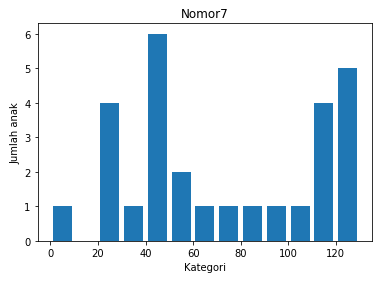
\includegraphics[width=9cm]{figures/6/Teori/1174056/7his.png}
    \caption{histogram}
    \centering
\end{figure}

\subsection{Jelaskan lebih mendalam tentang parameter dari fungsi pie diantaranya labels, colors, startangle, shadow, explode, autopct}
\begin{itemize}
    \item Labels = berfungsi untuk menampilkan tulisan pada diagram pie
    \item Colors = berfungsi untuk menentukan warna pada tiap bagian pada diagram pie
    \item Startangle = berfungsi untuk menentukan sudut pertama pada diagram pie
    \item Shadow = berfungsi untuk menampilkan efek timbul pada diagram pie
    \item Explode = berfungsi untuk menunjukkan jarak pisah dari diagram pie.
    \item Autopct = berfungsi umtuk menampilkan jumlah angka dibelakang koma pada bilangan pecahan
\end{itemize}

\subsection{Pengecekan Plagiarisme Teori}
\begin{figure}[H]
	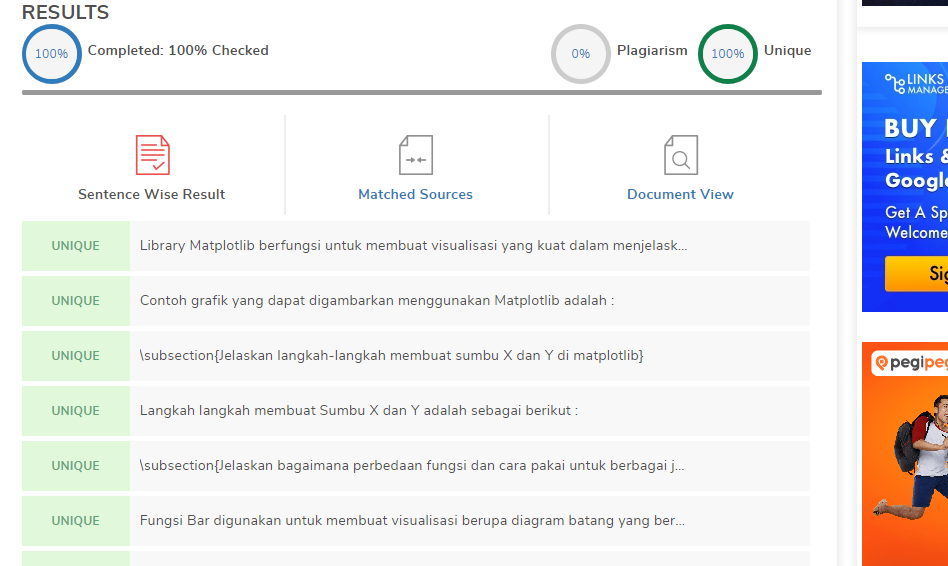
\includegraphics[width=9cm]{figures/6/Teori/1174056/Plagiat.png}
	\centering
\end{figure}